%
% The first command in your LaTeX source must be the \documentclass command.
\documentclass[sigchi]{acmart}

%
% defining the \BibTeX command - from Oren Patashnik's original BibTeX documentation.
\def\BibTeX{{\rm B\kern-.05em{\sc i\kern-.025em b}\kern-.08emT\kern-.1667em\lower.7ex\hbox{E}\kern-.125emX}}


\usepackage{amssymb}
\usepackage{amsmath}
\usepackage{algpseudocode}
\usepackage{algorithm}
\usepackage{tabularx}
\usepackage{enumerate}
\usepackage[inline]{enumitem}
\usepackage{subcaption}

\usepackage[flushleft]{threeparttable} % http://ctan.org/pkg/threeparttable
\usepackage{booktabs,caption}

\algnewcommand\algorithmicforeach{\textbf{for each:}}
\algnewcommand\ForEach{\item[ \algorithmicforeach]}
\algdef{S}[FOR]{ForEach}[1]{\algorithmicforeach\ #1\ \algorithmicdo}

% Rights management information. 
% This information is sent to you when you complete the rights form.
% These commands have SAMPLE values in them; it is your responsibility as an author to replace
% the commands and values with those provided to you when you complete the rights form.
%
% These commands are for a PROCEEDINGS abstract or paper.
\copyrightyear{2019}
\acmYear{2019}
\setcopyright{acmlicensed}
\acmConference[SNA '20]{Social Network Analysis '20}{2019/20}{University of Pisa, Italy}
\acmBooktitle{Social Network Analysis '20}
\acmPrice{0.00}
%\acmDOI{10.1145/1122445.1122456}
%\acmISBN{978-1-4503-9999-9/18/06}


% end of the preamble, start of the body of the document source.
\begin{document}

%
% The "title" command has an optional parameter, allowing the author to define a "short title" to be used in page headers.
\title{Microsoft OAG Network Analysis}

%
% The "author" command and its associated commands are used to define the authors and their affiliations.
% Of note is the shared affiliation of the first two authors, and the "authornote" and "authornotemark" commands
% used to denote shared contribution to the research.
\author{Marco Cardia}
\email{m.cardia@studenti.unipi.it}
\affiliation{%
  \institution{Student ID: 530567}
}

\author{Francesco Sabiu}
\email{f.sabiu@studenti.unipi.it}
\affiliation{%
  \institution{Student ID: 533231}
}

\renewcommand{\shortauthors}{Francesco Sabiu, Marco Cardia}


% The abstract is a short summary of the work to be presented in the article.
\begin{abstract}
The co-authorship of articles in learned journals provides several patterns of collaboration within the academic community. In this study, we collect the data related to the 2016 academic co-authorships and we build a network from them. We use these data along with several measures and algorithms in order to answer a broad variety of questions about the patterns they reveal.
After characterizing the network, we analyse it by means of different community discovery algorithms. Thus, we apply some Opinion Dynamics models in order to simulate the spreading of plausible innovations. Moreover, we find some correlations between network properties and authors' features. The achieved results described in our paper are available at the team GitHub repository
\footnote{
{\bf Project Repositories}\\
\noindent Data Collection: \url{https://github.com/sna-unipi/data-collection-2020_sabiu}\\
\noindent Analytical Tasks: \url{https://github.com/sna-unipi/network-analysis-analytical-tasks-2020_sabiu}\\
\noindent Report: \url{https://github.com/sna-unipi/project-report-2020_sabiu}}.
\end{abstract}


%
% Keywords. The author(s) should pick words that accurately describe the work being
% presented. Separate the keywords with commas.
\keywords{Social Network Analysis, Scale-Free Networks, Co-authorship}


%
% This command processes the author and affiliation and title information and builds
% the first part of the formatted document.
\maketitle

\section{Introduction}
Coauthorship of papers can be seen as a fact assessing the collaboration between two or more authors. From a more collective point of view, such data form a global network of collaboration, known in literature as co-authorship network.
Several studies of scientific networks have been published in bibliometrics and social network analysis: they investigate properties of different types of networks in which the nodes are usually papers \cite{papers}, authors \cite{Newman5200} or organizations \cite{organizations}. In our study, we analyse a network whose nodes are authors linked by their collaborations extracted from papers information, making use of Microsoft Open Academic Graph data. \\
Our contribution is twofold. Firstly, we construct the graph described by the adopted dataset and we analyse its topological properties in order to provide a structural understanding of the academic community. Secondly, we dig into a deeper analysis of the network by applying several state-of-the-art algorithms related to community discovery, link prediction and opinion dynamics. Finally, we investigate for interesting correlations among individual and collective properties of the network. \\
The rest of the paper is organized as follows. Section \ref{sec:dataCollection} provides a detailed implementation of the techniques and algorithms used for the collection of data from the Open Academic Graph provided by Microsoft \cite{AMiner1}\cite{AMiner2}, together with the description of the available data. In Section \ref{sec:networkCharacterization} we describe both the extracted network and the larger of its connected components by means of the typical measures and statistics that characterize networks, providing also a comparison with respect to the most known network models. Next, in Section \ref{sec:communityDiscovery} we apply, evaluate and compare four state-of-the-art algorithms with the purpose of individuating the communities composing the co-authorship network. In Section \ref{sec:linkPrediction} we describe the algorithms adopted for the link prediction task, their goal and the achieved results, while in Section \ref{sec:ODynamics} we do the same for five state-of-the-art algorithms adopted for the analysis of the opinion spreading within the network. Furthermore, in Section \ref{sec:CDweighted} we exploit the weights of the collected network by providing an implementation of an overlapping community discovery algorithm for weighted networks. In the same section, its description together with the evaluation of this application on the network are provided. Finally, we  answer several questions related to the authors. In particular, we try to discover pattern involving both the collective properties (communities, overall network characteristics) and the individual ones, such as the performance index of the authors or the number of citations and publications. The results of the investigation are presented in Section \ref{sec:openQuestion} and \ref{sec:discussion}. In the latter, we also highlight the main criticisms addressed in our work, as well as the reason of the described choices.   

\section{Data Collection}\label{sec:dataCollection}
In this section, the source data, as well as the steps involved in the extraction of relevant information from them, are described. After providing a brief characterization of the available data, we dig into the details of the methodology adopted for their manipulation, illustrating the most meaningful steps along with the raised criticisms.

\subsection{Selected Data Sources}\label{sec:dataSource}
Open Academic Graph (OAG)\cite{AMiner1}\cite{AMiner2} is a knowledge graph provided by Microsoft as a service to the research community. It unifies two billion-scale academic graphs: Microsoft Academic Graph (MAG) and AMiner, which are constantly evolving according to the exponential growth of research bibliography. In order to perform our analysis we selected the January 2019 snapshot of the OAG v2. \\
The data that we considered were included in the following files:
\begin{itemize}
\item \textit{AMiner papers}: a table containing 172,209,563 papers with their information.
\item \textit{AMiner authors}: a 113,171,945 entries table containing information regarding the authors.
\end{itemize}
For our purpose, we decided to consider only a subset of the columns of such tables. For the first, we took into account only the fields \textit{year} and \textit{authors}, necessary to extract only the IDs of authors whose collaboration took place in 2016. Concerning the second, we considered \textit{name}, \textit{h-index}, number of both \textit{publications} and \textit{citations}, the related list of \textit{organizations} and the \textit{research fields}. \\
A challenging aspect of the collection phase has been represented by the size of the analysed files: those containing papers' information occupy 177 GB, while the authors related ones have size slightly greater than 35 GB. For this reason, the algorithms performing the data collection tasks have followed a streaming approach.

\subsection{Extraction Methodology and Assumptions}
Due to the size of the files mentioned in section \ref{sec:dataSource}, the extraction of authors' IDs and authors' information has been performed in an online fashion. In particular, files have been read in chunks of 10000 entries in order to overcome to the gap between RAM capacity and data size. Such technique has been feasible because of the following property on the papers data P: no dependency with records $\neq i$ exists for each $i \in P$. \\
Algorithms \ref{alg:linkExtr} and 2 illustrate the developed algorithms. While the former obtains the list of relevant links from the AMiner papers table, the latter retrieves authors' information from AMiner authors table.

\begin{algorithm} \caption{Link extraction}\label{alg:linkExtr}
\begin{algorithmic}[1]
\Require $paper_i.txt$ to be in $papers/$ folder
\State Initialize $chunk\_size = 10000$, $links = \{\}$
\State $P = papers/*.txt$
\Repeat
    \State $paper = P.pop()$
    \Repeat 
        \State $C=readChunk(paper, chunk\_size)$
        \ForEach{$p \in \mathcal C $}
            \If{$ p.year == 2016 $}
                    \ForEach{pair $auths \in p.authors$}
                        \State $links = links \cup pair$
                    \EndFor
            \EndIf
        \EndFor
    \Until {$C \neq \{\}$}
\Until {$P \neq \{\}$}
\end{algorithmic}
\end{algorithm}

An observation is in order at this point. The goal of Algorithm \ref{alg:authExtr} is to retrieve information related to m over n total authors, with n >> m.
In a usual batch algorithm we would implement this task by performing m lookups in the n entries (both sets are unsorted). In our case, because of the online paradigm, we have to revert such approach: for each author whose information is stored, we look whether it is contained in the stored links. If yes, its information is fetched.

\begin{algorithm} \caption{Authors information extraction}\label{alg:authExtr}
\begin{algorithmic}[1]
\Require $links$ to be a set of pairs of valid authors IDs \\ 
        $authors_i.txt$ to be in $authors/$ folder
\State Initialize $chunk\_size = 10000$, $authors = \{\}$
\State $A = authors/*.txt$
\Repeat
    \State $author = A.pop()$
    \Repeat 
        \State $C=readChunk(author, chunk\_size)$
        \ForEach{$a \in \mathcal C $}
            \If{$ \exists pair \in links: a \in pair$}
                \State $authors = authors \cup a$
            \EndIf
        \EndFor
    \Until {$C \neq \{\}$}
\Until {$A \neq \{\}$}
\end{algorithmic}
\end{algorithm}

After the execution of Algorithms \ref{alg:linkExtr} and \ref{alg:authExtr} we have obtained the worldwide 2016 co-authorship network, made up of 373263 nodes and 4511734 links. \\
In the next sections, such network will be object of some analyses and comparisons. Notice that one or more sub-samples of it may be used to estimate some measures that otherwise would be computationally too expansive with respect to the adopted hardware
\footnote{
\noindent Data Collection has been performed by means of Google Colaboratory Reserch, providing n1-highmem-2 instance with 2vCPU @ 2.2GHz, 25GB of RAM and 110 GB of secondary memory. \\
Several algorithms for Link Prediction, Opinion Dynamics and Community Discovery have been executed on the AI Platform provided by Google Cloud Platform (n1-highmem-8 with 8 vCPUs, 52 GB RAM) and on Amazon AWS machines (4 CPUs, 32 GB RAM).
}. In particular, the majority of the tasks described in the following made use of the biggest connected component of the original graph. When used, this assumption will be specified in the related section.

\section{Network Characterization}\label{sec:networkCharacterization}
Let $B$ be a set of bibliographic entities such as scientific papers, journals, publications or books published in 2016. Let A be the set of authors appearing in $B$, and $coauthors(b, a_1, a_2)$ a predicate that is true if and only if both $a_1$ and $a_2$ appear in $B$ as authors. The co-authorship network corresponding to $B$ is the undirected weighted graph $G=(V, E)$ in which:
\begin{itemize}
    \item The set of nodes $V$ corresponds to the set of authors $A$.
    \item Two nodes $v_1$ and $v_2$ are connected by an undirected edge (link) $e \in E$ iff $ \exists b \in B$ : $coauthors(b, v_1, v_2) = true$, i.e. if and only if $b$ is jointly co-authored by $v_1$ and $v_2$.
    \item Each edge $e= \langle v_1,v_2,w \rangle$ is a tuple in which the weight $w = \# \{b \in B$ : $coauthors(b, v_1, v_2) = true\}$
\end{itemize}
Furthermore, network nodes are characterized by the following attributes:  \\
\begin{itemize}
    \item \textit{Name}: a non unique string containing the name of the author;
    \item \textit{h-index}: a number representing the \textit{de facto standard} author-level metric that measures both author's productivity and citation impact;
    \item \textit{Number of publications} of the author related to its publications up to 2016;
    \item \textit{Number of citations} of the author related to all the publications up to 2016;
    \item \textit{Organizations}: a list of the author's affiliated organizations up to according to OAG data source.
\end{itemize}

Since some of the following measures involve expansive computation, such as the one of the diameter, we perform them on the biggest connected component individuate in the connectedness analysis.

\subsection{On the degree distribution}
Once we have obtained the network, some consideration can be made about its structure. Firstly, as expected by the knowledge of the context, we have that $L_{max} = \frac{N(N-1)}{2} >> L$ and the average degree is 24, meaning that the network is sparse. 
Secondly, as shown in Figure \ref{fig:degreeDistribution}, the degree distribution follows the typical pattern of the Scale-Free networks, from which we can get the power law.

\begin{figure}[h]
  \centering
  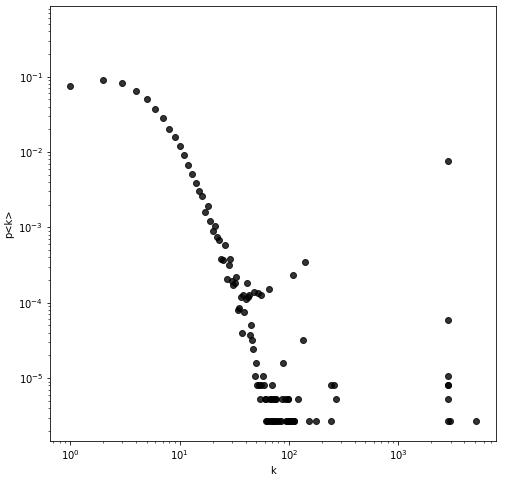
\includegraphics[width=\linewidth]{report/img/degreeDistribution.png}
  \caption{Co-authorship network degree distribution}
  \label{fig:degreeDistribution}
\end{figure}

\subsection{Connectedness}
Given the context that we are analysing, one could expect the network to made up by several connected components: since researchers tend to interact with other researcher of the same field such components could depend on the research fields, or on geographical attributes for example. In order to fact-check this intuition we have performed a connected components analysis, whose quantitative results are illustrated in Figure \ref{fig:componentDistribution}. In the log-log plot, the distribution of the size of the connected components is provided: expectedly, it follows the same pattern of the degree distribution, confirming the scale-free nature of the network.

\begin{figure}[ht]
  \centering
  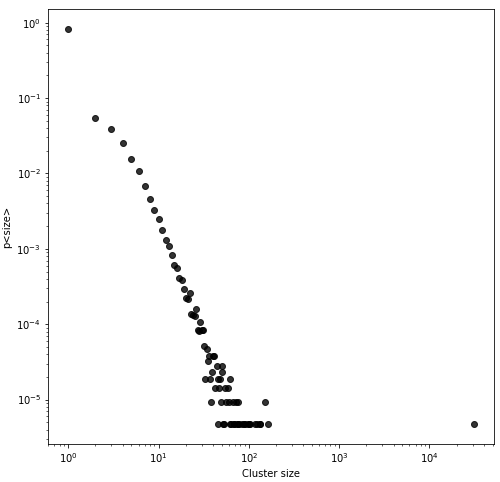
\includegraphics[width=\linewidth]{report/img/componentDistribution.png}
  \caption{Co-authorship network connected components size distribution}
  \label{fig:componentDistribution}
\end{figure}

Figure \ref{fig:componentDistribution} highlights the presence of a particular connected component: its size is between 2 and 3 orders of magnitude greater than both mean and median of the other cluster sizes. \\
In the following subsection, we perform some analyses on such cluster, since it represent the only connected component made up of more than some hundreds nodes. Other components of approximately mean size will be analyzed, as well.


\begin{table}
  \caption[Connected components degrees with respect to the network]{Connected components degrees with respect to the network}
  \label{tab:connected_components_degree}
  
\begin{threeparttable}
  \begin{tabular}{lcc}
    \toprule
    Component & Avg degree & Max degree\\
    \midrule
    Full network    & 24 & 5134\\
    Biggest component & 50  & 5136\tnote{*} \\
    All others (max) & 29    & 66 \\
    All others (avg) & 0.48    & 0.57 \\
  \bottomrule
\end{tabular}
\begin{tablenotes}
    \begin{flushleft}
      \item[*] We consider this result incongruent with respect to the maximum degree detected in the whole network, that is lower.
    \end{flushleft}
\end{tablenotes}
\end{threeparttable}
\end{table}


\subsection{Path analysis}
Since many connected components compose the graph, its diameter and average path length are infinite. Hence, we have performed the path analysis on the sub-graph identified in the previous section, that was expected to represent an upper bound (for such path-related measures) with respect to the other clusters. We discovered that its diameter and path length are actually greater than those of the others clusters, confirming that the network structure follows the same pattern within each connected component.\\

\begin{table}
  \caption{Connected components paths comparison among full network, biggest component and all other components}
  \label{tab:connected_components_paths}
  \begin{tabular}{lcc}
    \toprule
    Component & Diameter & Avg path length\\
    \midrule
    Full network    & $\infty$ & $\infty$\\
    Biggest component & 50  & 11.32\\
    All others (max) & --\tnote{*}    & 6.99 \\
    All others (avg) & --\tnote{*}    & 1.08 \\
  \bottomrule
\end{tabular}
\begin{tablenotes}
\begin{flushleft}
  \item[*] The computations required too much time.
\end{flushleft}
  \end{tablenotes}
\end{table}

\subsection{Clustering coefficient and density analysis}
By definition, co-authorship networks are made up of groups of authors related each other by one or more article. From a topological point-of-view, their nature leads the network to be composed by a chain of cliques, ideally representing research groups. Such property is reflected in the value of the global clustering coefficient of the network, obtained as follows:
$$ C_{network} = \frac{\sum_{i=1}^{n} \frac{2\times L_{i}}{ k_i(k_i-1)}}{n}$$
where:
\begin{itemize}
    \item $L_i$ is the maximum number of existing links among the neighbors of the node $i$.
    \item $k_i$ is the number of neighbors of the node $i$, thus the term $k_i(k_i -1)$ represents the maximum number of possible links (fully connected network) among them. 
\end{itemize}
We calculated the global clustering coefficient for both the biggest connected component and the whole graph, obtaining almost equivalent values: 0.998. This information confirms the expected network structure, in which we have cliques-like networks composing each cluster.

Concerning the graph density, we also evaluated it separately for the whole graph and for its biggest connected component. They differed for several orders of magnitude: the whole network density is indeed $6 \times 10^{-5}$, while the one of the biggest connected component is $8 \times 10^{-3}$. We can conclude that the considered subgraph is quite denser than the rest of the network. 

\subsection{Centrality analysis}
We performed the network centrality analysis by applying the classic network centrality measures used in literature, namely betweenness centrality, closeness centrality, degree centrality and eigenvector centrality. All of the following centrality measures have been computed by means of the Python \textit{igraph} library \cite{csardi2006igraph}. 

\subsubsection{Betweenness centrality}
The betweenness centrality of a node is a measure of its centrality based on shortest paths. Indeed, it is informally defined as the number of shortest paths between every possible pair of nodes passing for it. More formally, it is defined as follows.

\begin{definition}
\textit{(Betweenness centrality)} \\
Given a network $G=(V, E)$ with $|V| = n$ and $|E| = m$, its average betweenness centrality is defined as 
$$ C_b(i) = \sum_{j \neq k} \frac{\sigma_{jk}(i)}{\sigma_{jk}}$$
where 
\begin{itemize}
    \item $\sigma_{jk}(i)$ is the number of geodesic paths from j to k via i;
    \item $\sigma_{jk}$ is the number of geodesic paths from j to k.
\end{itemize}
\end{definition}

\subsubsection{Degree centrality}
This measure is defined on the base of the number of links incident upon a node, also known as grade of the node itself. It is the most basic measure since it relies on a local property. Formally, we define it in the following way.

\begin{definition}
\textit{(Degree centrality)} \\
Given a network $G=(V, E)$ with $|V| = n$ and $|E| = m$, the degree centrality of a node $i$ is defined as
$$ k_i(i) = \sum_{j = 1}^{n} A_{ij}$$
where $A$ is the adjacency matrix of $G$.
\end{definition}

\subsubsection{Closeness centrality}
Intuitively, closeness centrality measures how close a vertex is to all other vertices in the graph. Its value is obtained calculating the reciprocal of the sum of the length of the shortest paths between the node and all other nodes in the graph \cite{closeness}. In formulas, we define it as follows.

\begin{definition}
\textit{(Closeness centrality)} \\
Given a network $G=(V, E)$ with $|V| = n$ and $|E| = m$, its closeness centrality of a node $i$ is defined as 
\begin{equation}
    C_{cl}(i) = \frac{n-1}{\sum_{d_{ij < \infty}} d_{ij}}     
\end{equation}

where $d_{ij}$ is the distance between the nodes $i$ and $j$ of $G$.
\end{definition}

\subsubsection{Eigenvector centrality}
Eigenvector centrality measures the importance of a node in the network. After initializing initial scores, the algorithm give importance to a node if it is linked to other nodes, depending on the importance of its neighbors. More formally, we can define it as follows.

\begin{definition}
\textit{(Eigenvector centrality)} \\
Given a node $u$ belonging to a network $G=(V, E)$ with $|V| = n$ and $|E| = m$, the centrality score of a node $i$ is defined as follows: 
$$ x_{i}^{(t+1)}= \sum_{j=1}^{n} A_{ij}x_{j}{(t)}$$
where $x_{i}$ is the centrality of the node $i$.
\end{definition}

From the application of the above defined centrality measures, we find that almost all of their distributions follow an exponential pattern. This is a direct consequence of the network structure. Figure \ref{fig:centralities} graphically illustrates such results. Notice that the eigenvector centrality values have been logarithmically scaled.

\begin{figure}[]
\begin{subfigure}{.45\columnwidth}
  \centering
  % include first image
  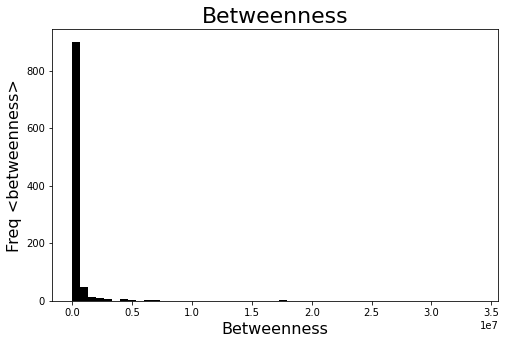
\includegraphics[width=\columnwidth]{report/img/betw.png} 
  \caption{Betweenness centrality}
  \label{fig:sub-bet}
\end{subfigure}
\hfill
\begin{subfigure}{.45\columnwidth}
  \centering
  % include second image
  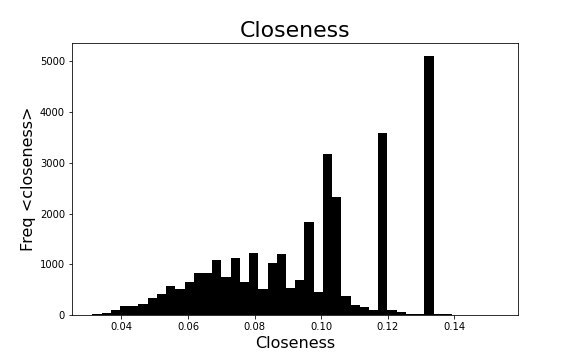
\includegraphics[width=\columnwidth]{report/img/clos.jpg}
  \caption{Closeness centrality}
  \label{fig:sub-clo}
\end{subfigure}
\hfill
\label{fig:centralities}
\caption{Centrality measures distribution calculated over the biggest component.}

\begin{subfigure}{.45\columnwidth}
  \centering
  % include first image
  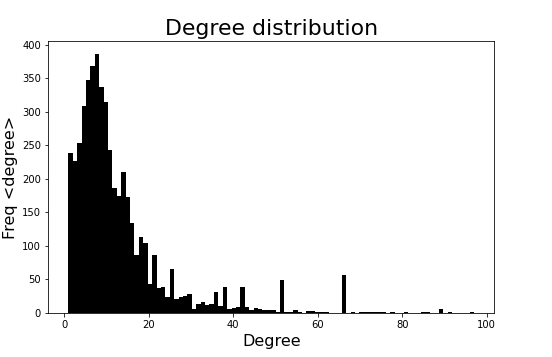
\includegraphics[width=\columnwidth]{report/img/degr.png} 
  \caption{Degree centrality}
  \label{fig:sub-deg}
\end{subfigure}
\hfill
\begin{subfigure}{.45\columnwidth}
  \centering
  % include second image
  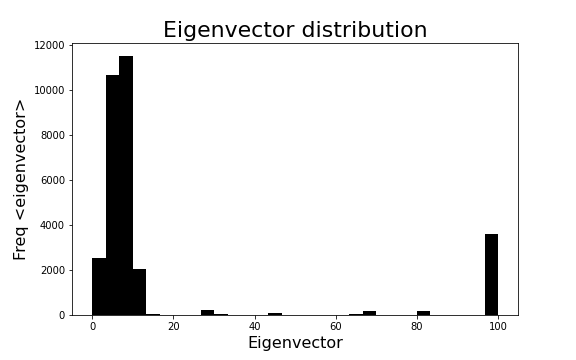
\includegraphics[width=\columnwidth]{report/img/eigen.png}
  \caption{Eigenvector centrality}
  \label{fig:sub-eig}
\end{subfigure}
\hfill
\label{fig:commCorrelation}
\caption{Centrality measures distribution calculated over the biggest component.}
\end{figure}


\subsection{Comparison with network models}
As a matter of fact, we provide a brief comparison among our network and the most known models existing in literature, namely Erdős–Rényi (ER)\cite{Erdos1959}, Barabási–Albert (BA)\cite{Barabasi509} and Watts–Strogatz (WS)\cite{Watts-Colective-1998}. Intuitively, such models generalize networks whose nodes respectively form \begin{enumerate*}[label=(\roman*)]
    \item a random network
    \item a configuration model
    \item a (random) scale-free network and 
    \item a small-world network
\end{enumerate*}. Nodes collective behaviour (i.e. their emergent properties in terms of link to other nodes) can be expressed more accurately by means of a set of structural network measures such as degree distribution, path length and clustering coefficient. With this purpose, we firstly provide an informal description summarizing such properties for the three models (Table \ref{tab:netProperties}). Next, we formalize them in Table \ref{tab:netFormulas} by means of formulas which are function of the number of nodes and links.

\begin{table}
  \caption{Order of magnitude of topological measures for ER, BA and WS models}
  \label{tab:netProperties}
  \resizebox{\columnwidth}{!}{%
  \begin{tabular}{lccc}
  \hline
    Network & Degree distribution & Path length & Clustering coefficient\\
    \hline
    \begin{tabular}{@{}l@{}} Erdős–Rényi \\(Random Network) \end{tabular} & Poissonian & Short & Small\\
    
    Configuration model &
    \begin{tabular}{@{}c@{}} Custom,\\ can be broad
    \end{tabular} & Short & Small \\
    
    \begin{tabular}{@{}l@{}} Watts–Strogatz (WS) \\(small world)
    \end{tabular} & Poissonian & Short & Large \\
    
    \begin{tabular}{@{}l@{}} Barabási–Albert \\(Scale-free)     \end{tabular} & Power-law & Short & Rather small\\
    \hline
\end{tabular}}
\end{table}


\begin{table}
  \caption{Models topological measures with parameters}
  \label{tab:netFormulas}
  \resizebox{\columnwidth}{!}{
  \begin{tabular}{lccc}
    \toprule
    Network & Degree distribution & Path length & Clustering coefficient\\
    \midrule
     \begin{tabular}{@{}l@{}}Erdős–Rényi \\(Random Networks) \end{tabular} & $p_k=\frac{\langle k \rangle ^k}{k!}e^{-\langle k \rangle}$ & $\mathcal{O}(log(N))$ & $C_i = \frac{\langle k \rangle}{n-1}=p$\\ 
     
     Configuration model & $p_{nei,k} = \frac{kp_k}{\langle k \rangle}$ & $\mathcal{O}(log(N))$ & $C=\frac{1}{n} \frac{[\langle k \rangle^2 - \langle k \rangle ]^2}{\langle k \rangle ^3}$ \\
     
     \begin{tabular}{@{}l@{}} Watts–Strogatz (WS) \\(small world) \end{tabular} & $P(k) = e^{-Kp} \frac{(Kp)^{k-K}}{(k-K)!}$ & $\frac{ln(nKp)}{K^2p}$ & $\frac{3(K-2)}{4(K-1)+8Kp +4Kp^2}$ \\
     
     \begin{tabular}{@{}l@{}}Barabási–Albert \\(Scale-free) \end{tabular} & $P(k) \sim Ck^{-\gamma}$ & $\frac{lnN}{lnlnN}$ & $\frac{m}{4} \frac{(lnN)^3}{N}$\\
     
  \bottomrule
\end{tabular}}
\end{table}

For the comparison of our network with the cited models, we proceeded as follows. Firstly, in order to get the distribution we exploit NetworkX Python library \cite{networkX} to create the graphs according to the network models of Table \ref{tab:netFormulas}. Then, we calculated the statistics reported in the previous subsection for each of these models. In particular, we focused on degree, average path length and clustering coefficient. The results of this analysis are reported in Table \ref{tab:modelsComparison}, in which we compare our network statistics with the one of the studied models. Where values are infinity, we substitute them with the same measures applied to graphs having the same size of the biggest subgraph of ours. 

\begin{table}
  \caption{Comparison among network models and co-authorship network}
  \label{tab:modelsComparison}
  \resizebox{\columnwidth}{!}{%
  \begin{tabular}{lccc}
  \hline
    Network & Degree distribution & Path length & Clustering coefficient\\
    \hline
    \begin{tabular}{@{}l@{}} Erdős–Rényi model \end{tabular} & Fig. \ref{fig:sub-er} & 10.35 &  $6.48 \times 10^{-5}$\\
    
    Configuration model & Fig. \ref{fig:sub-conf} & 10.35 & $1 \times 10^{-4}$ \\
    
    Watts–Strogatz (WS) & Fig. \ref{fig:sub-ws} & 1 & 0.08 \\
    
    Barabási–Albert & Fig. \ref{fig:sub-ba} & 4.43 & $1 \times 10^{-3}$ \\
     
     Co-authorship network \\ (subgraph) & Fig. \ref{fig:degreeDistribution}. & 24 & 0.998 \\
    \hline
\end{tabular}}
\end{table}

\begin{figure}[]
\begin{subfigure}{.45\columnwidth}
  \centering
  % include first image
  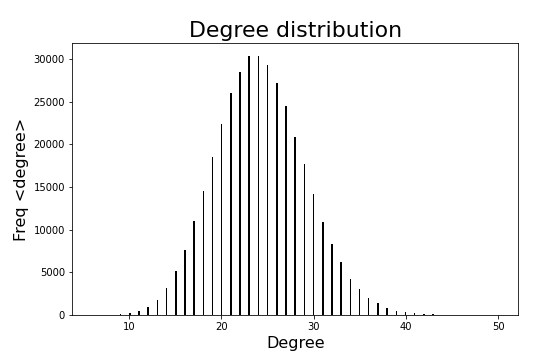
\includegraphics[width=\columnwidth]{report/img/er_degr.png} 
  \caption{Erdős–Rényi}
  \label{fig:sub-er}
\end{subfigure}
\hfill
\begin{subfigure}{.45\columnwidth}
  \centering
  % include second image
  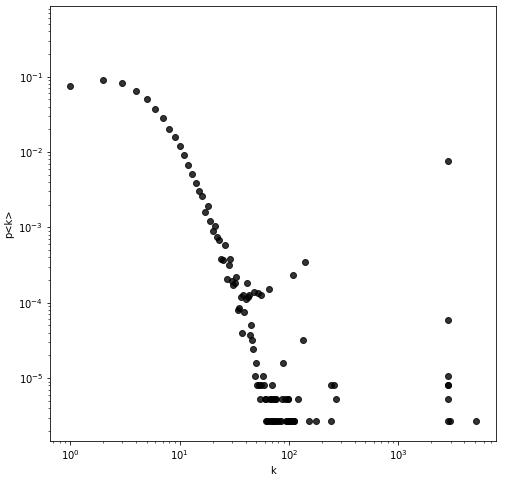
\includegraphics[width=\columnwidth]{report/img/degreeDistribution.png}
  \caption{Configuration model}
  \label{fig:sub-conf}
\end{subfigure}
\hfill
\begin{subfigure}{.45\columnwidth}
  \centering
  % include second image
  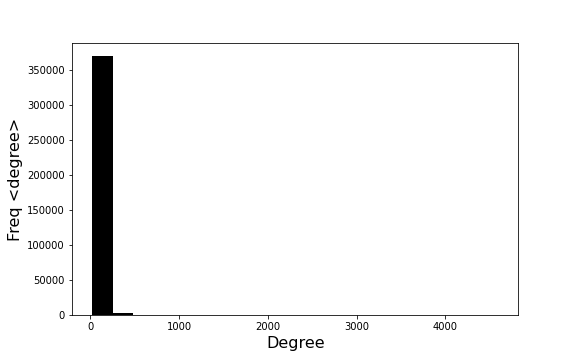
\includegraphics[width=\columnwidth]{report/img/ba_degr.png}
  \caption{Barabási–Albert}
  \label{fig:sub-ba}
\end{subfigure}
\hfill
\begin{subfigure}{.45\columnwidth}
  \centering
  % include second image
  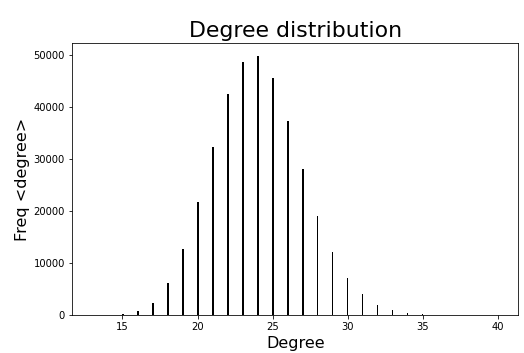
\includegraphics[width=\columnwidth]{report/img/ws_degr.png}
  \caption{Watts–Strogatz}
  \label{fig:sub-ws}
\end{subfigure}
\hfill
\label{fig:commCorrelation}
\caption{Correlation between community properties and authors' features.}
\end{figure}

\section{Community discovery}\label{sec:communityDiscovery}
In this section, several Community Discovery (CD) approach are described, and applied. A description of their result is also provided. Each applied algorithm corresponds to a different technique having as goal the detection of similar authors of the network. 
Depending on the algorithm, similarity can refer either to the network structure or to the node features. \\
We applied some of the algorithms provided by the Python library CDlib \cite{rossetti:hal-02197272}, that allows all extraction, comparison, and evaluation of communities from complex networks. The algorithms we run are Label Propagation \cite{label}, Louvain \cite{Blondel_2008}, K-clique ($k=3$) \cite{kclique} and Demon ($\epsilon=0.25$) \cite{Coscia2012DEMONAL}. Concerning the last, we had to choose between it and Angel \cite{angel} because they were the two most computational expansive.
We evaluated the discovered communities by means of four evaluation functions among those provided by CDlib, namely Internal Edge Density \cite{intEdgeDensity}, Average Internal Degree \cite{avgIntDegree}, Modularity Density \cite{modDensity} and Conductance \cite{conductance}. Table \ref{tab:CDscores} shows the resulting scores. Notice that the k-Clique algorithm returns the same results in terms of evaluation for each of the following values of the parameter $k$ (representing the size of smallest clique): 3, 5 and 7. This implies that each of the detected communities has size greater or equal to 7.

\begin{table}[ht!]
  \caption{Community Discovery algorithms evaluation}
  \label{tab:CDscores}
  \resizebox{\columnwidth}{!}{
  \begin{tabular}{lcccc}
    \toprule
    Evaluation & Label Propagation & Louvain & k-Clique & Demon \\
    \midrule
    Internal Edge Density & 0.19 & 0.08 & \textbf{0.23} & 0.17\\
    Average Internal Degree & 5.38 & \textbf{78.16} & 5.14 & 10.02\\
    Modularity Density & \textbf{1106.91} & 10.01 & -59631.28 & -17937.91\\
    Conductance & 0.25 & \textbf{0.06} & 0.46 & 0.38\\
  \bottomrule
\end{tabular}}
\end{table}

Some considerations are in order at this point. At first glance, we observe significant differences among the modularity values applied to the communities discovered by the three algorithms. In particular, the k-Clique algorithm produces (together with Demon) low-modularity communities. Instead, modularity is maximized by Label Propagation, resulting the best approach for a such dense network. \\
Also the conductance measure is importantly affected by the applied algorithm, that impact on this measures. Results range in one order of magnitude, from $10^{-2}$ to $10^{-1}$, having best values for the communities discovered by means of \textit{Label Propagation} and \textit{Louvain}. 
Similarly, the average node degree of the communities is optimized (i.e. maximized) by \textit{Louvain}, while k-Cliques optimizes the Internal Edge Density: this result is reasonable and expected, since k-Cliques creates communities starting from adjacent k-cliques.

\section{Link prediction} \label{sec:linkPrediction}
Link prediction algorithms are applied to networks for several purposes: for example, they can provide missing information from incomplete networks, identify their evolving mechanisms or find future or spurious interactions. Depending on their approach, they can be supervised or unsupervised. In our analysis, we applied the following four unsupervised link prediction algorithms to the biggest connected component extracted from the starting network.
\begin{itemize}
    \item \textit{Common neighbors} \cite{commonNeighbors}, in which the correlation between the size of the common neighborhood between two nodes and the probability of a their future connection is exploited.
    \item \textit{Jaccard} \cite{Jaccard}, that is based on the Jaccard similarity, i.e. a set similarity measure widely adopted in Information Retrieval since 1980s. In this link prediction algorithm, it is applied on the features of two nodes, relying on the assumption that the more portion of features two nodes share, the more they are likely to create a relationship.
    \item \textit{Academic-Adar} \cite{AdamicAdar}: conceptually it is equivalent to the Jaccard-based one, since it makes use of nodes features to compare them. Its novelty relies on the computation of such similarity: rarer features (i.e. low frequency ones) are considered more important than the more frequent ones, contributing with a stronger weight in the calculation.
    \item \textit{Preferential attachment}: this category of algorithms is based on the fact that the probability of a new link for a node is proportional to the size of its neighborhood. This observation comes from \cite{BARABASI2002590}, in which authors shown the positive correlation between the link probability of two nodes and the product of their neighborhoods sizes.
\end{itemize}
We chose such algorithms because they reflect quite realistically the behavioural model that a co-authorship network could adopt. Indeed, if two researcher share a significant number of colleagues or research topics (common neighbors and features similarity) this fact increases the probability that they write a paper together. Contrarily, if they don't share neither a research group nor a research interest, it is reasonable to considerate such probability near to zero. The same reasoning applies for the preferential attachment -based predictions. \\
We availed ourselves of both linkpred and and NetowrkX \cite{networkX} Python libraries for all the prediction algorithm described in this section. For the sake of presentation, we applied them to the 9\textsuperscript{th} and 10\textsuperscript{th} biggest communities discovered by means of Louvain algorithm, since the application to the whole graph would be computational unsustainable for our resources. Nonetheless, only the results of the application of the Jaccard model is available. The rest of the algorithm are not available due to their execution time. Indeed, co-authorship networks are very dense networks, in which applying such kind of algorithms results time expensive. Concerning the Jaccard model, it returned a precision of 0.97 and recall value of 0.20 for the prediction. The graphical output of its evaluation is reported in Figure \ref{fig:jaccardEval}.\\

\begin{figure}[ht]
  \centering
  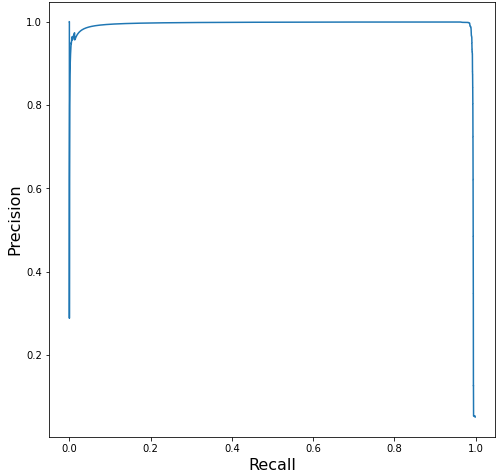
\includegraphics[width=0.8\linewidth]{report/img/jaccard.png}
  \caption{Evaluation of link prediction based on Jaccard model.}
  \label{fig:jaccardEval}
\end{figure}

For the explained reasons, in order to achieve the purposes of the present work, we applied to our network some Network Diffusion algorithms that are described in the next section. Contrarily to the link prediction algorithms, they don't rely on the analysis of each possible link of the network. Instead, they visit nodes just a constant number of time.

\section{Opinion Dynamics} \label{sec:ODynamics}
In this section, several applications of Opinion Dynamics algorithm are described. For the sake of example, one could imagine an opinion in a co-authorship network as a tool, idea or methodological innovation involving a research field. In the following presentation of diffusion algorithms, we abstract from the specific innovation and we apply algorithms taking into account the more possible generic meaning of opinion. \\
In the next paragraphs we compare several algorithms executed with several initial configurations and parameters. They take into account both discrete and continuous opinions. The considered models are Voter, Q-Voter, Majority Rule, Sznajd and Deffuant. In order to understand the obtained results and the differences among them, a concise description of them is reported in the following. 
\begin{itemize}
    \item \textit{Voter} \cite{voter} is a discrete Opinion Dynamics model in which an agent opinion changes if it is randomly selected. The new opinion of it will be the one of one of its neighbors.
    \item \textit{Sznajd} \cite{SznajdWeron2000OpinionEI} introduces the concept of group, considering the opinion of a collectivity more influential than the ones of single individuals. Indeed, two random-selected neighbors spread their opinion to their neighbors if they share the same opinion. Otherwise, the opposite effect is produced.
    \item \textit{Q-Voter} \cite{qvoter} combine the ideas of the previous two models: $q$ neighbors are randomly selected, and if they agree they influence another random neighbor opinion.
    \item \textit{Majority rule} \cite{majority}: based on the opinion dynamics that characterizes public debates, it assumes that in a random group individuals take the majority opinion within the group.
    \item \textit{Deffuant} \cite{deffuant} is a continuous model that takes into account the interaction between pairs of individuals. Depending on their open-mindness, two individuals can change their opinion. Their new opinion at the new iteration result the average of their opinion at the previous one.
\end{itemize}
For all the described models we availed ourseleves of the functions provided by the Python library NDlib (Network Diffusion) \cite{ndlib}. Concerning the last of the described models, we implemented it by means of the Algorithmic Bias algorithm \cite{AlgorithmicBias}, whose implementation is provided by such library (released in NDlib 4.0.1). Indeed, the results of the application of the Deffuant model correspond to the execution of Algorithmic Bias algorithms with parameter $gamma = 0$.

\subsection{Experiments}
The algorithms implementing all the mentioned models have been executed with several parameters, varying both the initial condition and the algorithms iterations. 
%Parameters
For each of the algorithm, the initial population characterized by the new opinion (i.e. \textit{fraction\_infected} parameter) has been 0.1, 0.3, 0.4 and 0.5. Concerning Majority Rule and Q-Voter, we also varied the $q$ parameter, from 3 to 7, with an increment of 2.
%Results
Table \ref{tab:ODconfigs} illustrates the algorithms executions performed on the network. For each execution we got both the trend and the prevalence graphics, by which we could evaluate and discuss the diffusion of the opinions. 

\begin{table}
  \caption{Opinion Diffusion algorithms configurations}
  \label{tab:ODconfigs}
  \begin{tabular}{lccc}
    \toprule
    Algorithm & Initial opinion spreading & q & iterations\\
    \midrule
    Voter & 0.1, 0.3, 0.4, 0.5 & - & 1500\\
    Q-Voter & 0.1, 0.3, 0.4, 0.5 & 3, 5, 7 & 1500 \\
    Sznajd & 0.1, 0.3, 0.4, 0.5 & - & 1500\\
    Majority rule & 0.1, 0.3, 0.4, 0.5 & 3, 5, 7 & 1500\\
  \bottomrule
\end{tabular}
\end{table}

In addition to the configuration of Table \ref{tab:ODconfigs}, we executed Deffuant algorithm varying the \textit{fraction\_infected} (0.15 and 0.25) and \textit{epsilon} (0.30 and 0.40) parameters. Figure \ref{fig:ODresults} shows the most relevant outcomes of such executions. 

\begin{figure*}[ht]
\begin{subfigure}{.20\textwidth}
  \centering
  % include first image
  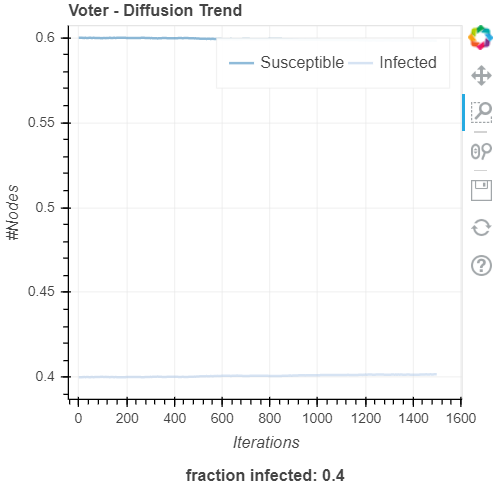
\includegraphics[width=\linewidth]{report/img/voter1.png}  
  \caption{Voter: 0.4 init.}
  \label{fig:sub-first}
\end{subfigure}
\hfill
\begin{subfigure}{.20\textwidth}
  \centering
  % include second image
  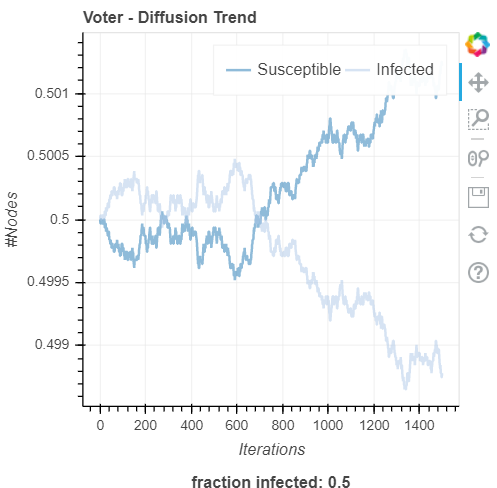
\includegraphics[width=\linewidth]{report/img/voter2.png}  
  \caption{Voter: 0.5 init.}
  \label{fig:sub-second}
\end{subfigure}
\hfill
\begin{subfigure}{.20\textwidth}
  \centering
  % include second image
  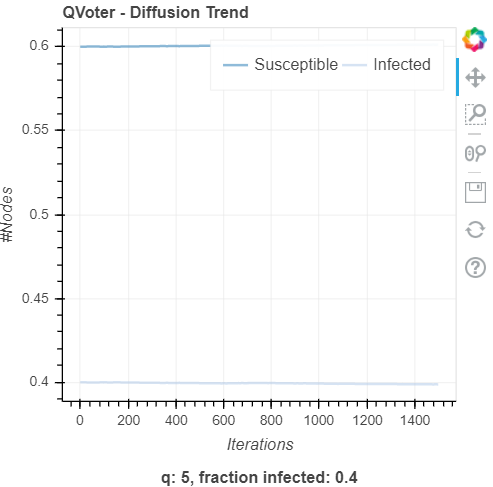
\includegraphics[width=\linewidth]{report/img/qvoter1.png} 
  \caption{Q-Voter: 0.4 init.}
  \label{fig:sub-third}
\end{subfigure}
\hfill
\begin{subfigure}{.20\textwidth}
  \centering
  % include second image
  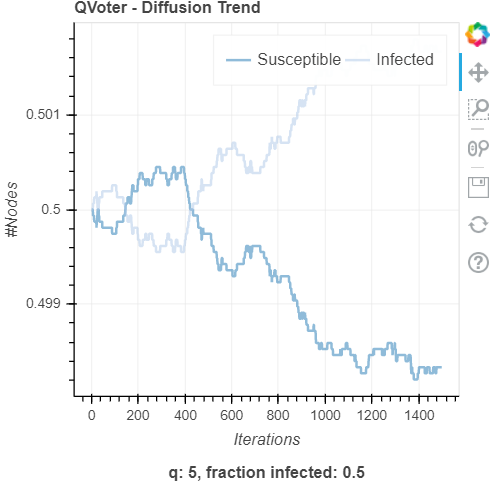
\includegraphics[width=\linewidth]{report/img/qvoter2.png} 
  \caption{Q-Voter: 0.5 init.}
  \label{fig:sub-fourth}
\end{subfigure}
\begin{subfigure}{.20\textwidth}
  \centering
  % include first image
  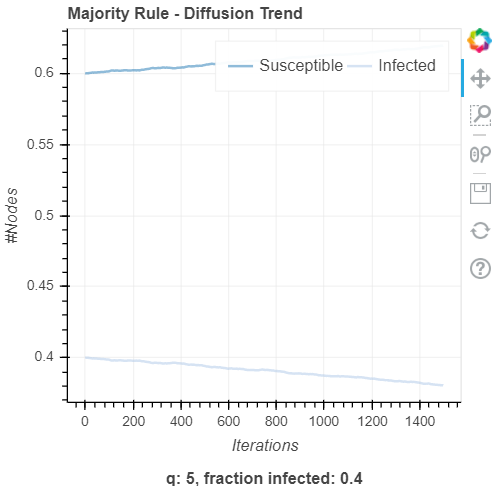
\includegraphics[width=\linewidth]{report/img/majority1.png}  
  \caption{Majority Rule: 0.4 init.}
  \label{fig:sub-fifth}
\end{subfigure}
\hfill
\begin{subfigure}{.20\textwidth}
  \centering
  % include second image
  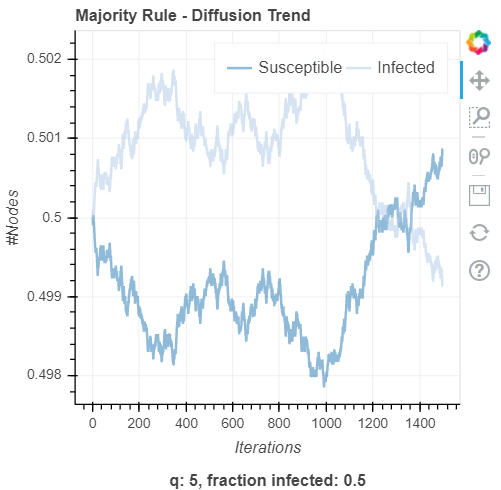
\includegraphics[width=\linewidth]{report/img/majority2.png}  
  \caption{Majority Rule: 0.5 init.}
  \label{fig:sub-sixth}
\end{subfigure}
\hfill
\begin{subfigure}{.20\textwidth}
  \centering
  % include second image
  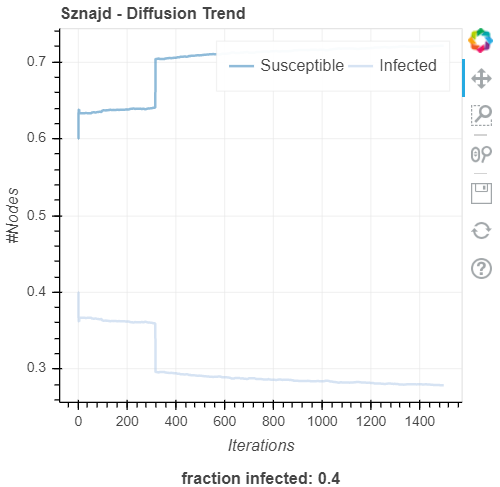
\includegraphics[width=\linewidth]{report/img/sznajd1.png} 
  \caption{Sznajd: 0.4 init.}
  \label{fig:sub-seventh}
\end{subfigure}
\hfill
\begin{subfigure}{.20\textwidth}
  \centering
  % include second image
  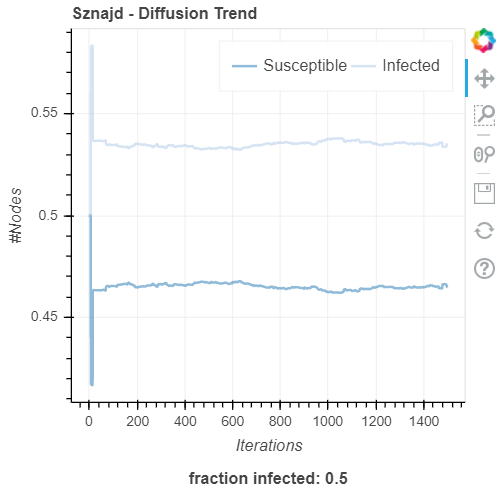
\includegraphics[width=\linewidth]{report/img/sznajd2.png}
  \caption{Sznajd: 0.5 init.}
  \label{fig:sub-eighth}
\end{subfigure}
\caption{Results of the opinion dynamics algorithms.}
\label{fig:ODresults}
\end{figure*}

For all the executions reported in Figure \ref{fig:ODresults} we executed 1500 iterations. Only 300 have been executed, instead, for Deffuant algorithm executions, by which we didn't get significant results. As we can observe from subfigures \ref{fig:sub-first}, \ref{fig:sub-third}, \ref{fig:sub-fifth} and \ref{fig:sub-seventh}, low initial values (lower than 0.5) do not lead to an important spreading within the given number of iteration. Contrarily, subfigures \ref{fig:sub-second}, \ref{fig:sub-fourth}, \ref{fig:sub-sixth} do reveal more interesting patterns: in two of the three cases, the infected individuals (i.e. authors reached by the innovation, in our study case) prevail within the first 1500 iterations. Finally, with Sznajd a different pattern is followed, since the number of susceptible and infected tends to the stability after a few dozens of iterations.

\section{Community Discovery in weighted networks} \label{sec:CDweighted}
Canonical Community Discovery algorithms such as those applied in Section \ref{sec:communityDiscovery} do not exploit network weights. Nonetheless, they can reveal additional information about communities. Thus, we analysed and implemented a local, efficient algorithm for detecting communities in weighted networks \cite{2010PhyA..389.4177C}. By means of it, we are also able to find overlapping communities, that are quite frequent in co-authorship networks, since an author can belong to different research groups during its career.

\subsection{Adopted measures}
The community detection technique adopted by the chosen algorithm \cite{2010PhyA..389.4177C} mainly exploits three measures regarding both nodes and community, namely \textit{Node Strength}, \textit{Belonging degree} and \textit{$Q_0$ Modularity}. In order to keep our paper self-contained, we provide their definitions together with a brief description of the authors method. While node strength is a local property, belonging degree and \textit{$Q_0$ Modularity} take into account respectively the community of the node and the whole graph.

\begin{definition}
\textit{(Node strength)} \\
Given a node $u$ belonging to a network $G=(V, E)$ with $|V| = n$ and $|E| = m$, its node strength is defined as 
$$ k_u = \sum_{v \in V} w_{uv}$$
where $w_{uv}$ is the weight of the edge $e_{uv}$, that is 0 if the edge does not exist. Intuitively, it represent its weighted degree, since it is obtained as the sum of the weights of its links.
\end{definition}

\begin{definition}
\textit{Belonging degree} \\
Given a node $u$ belonging to a community $C$, the belonging degree $B(u, c)$ is defined as
$$ B(u, C) = \frac{\sum_{v \in C} w_{uv}}{k_u}$$
where $w_{uv}$ is the weight of the edge $e_{uv}$, that is 0 if the edge does not exist. Less formally, the belonging degree of a node with respect to a community takes into account both the absolute node strength and the portion of it deriving from nodes of the same community. It is easy to demonstrate that this value is always between $[0, 1]$. 
\end{definition}

Finally, the algorithm proposed in \cite{2010PhyA..389.4177C} needs a measure that quantifies the strength of division of the network into communities. Authors adopt the following measure derived by the one proposed in \cite{modularity}. In such a way, the discovery algorithm can be also adopted for overlapping networks, since adopting $Q_0$ Modularity the algorithm doesn't suffer the resolution limit \cite{Fortunato2007ResolutionLI}.

\begin{definition}\label{def:modularity}
\textit{$Q_0$ Modularity} \\
Given a network $G=(V, E)$, the adjacency matrix $A$ and its set $C$ of communities, the $Q_0$ modularity is defined as follows: 
$$ Q_0 = \frac{1}{2m} \sum_{c \in C} \sum_{u,v \in V} \alpha_{cu} \alpha_{cv} \left( A_{uv} - \frac{k_u k_v}{2m} \right) $$
where $a_{cu}$ is a belonging coefficient defined as follows 
$$ \alpha_{cu} = \frac{k_{cu}}{\sum_{c \in C} k_{cu}}$$ and satisfying the condition $0 \le \alpha_{cu} \le 1,  \forall c \in C, u \in V $. Furthermore, we have that 
$k_{cu} = \sum_{v \in C} w_{uv}$. \\
In this way, the belonging coefficient includes the possibility of a node to be assigned to more communities and its definition is consistent with the one of modularity for a non-overlapping community \cite{modularity}.
\end{definition}

\subsection{The algorithm}
The implemented strategy for the detection of overlapping communities in weighted networks is composed by iterations of two  main steps, namely \textit{detection of the initial community} and \textit{expansion of the community}. Although all the implementation details are available at our mentioned GitHub repository, we describe the key steps of both phases. The following steps are iterated until every node belongs at list to a community. For this, an initialization procedure in which all nodes are labeled is performed.

\subsubsection{Detection of the initial community}
The initial community is detected among the non-labeled nodes. It starts from the strongest node (w.r.t. above defined node strength measure) and it spreads over its neighbors respecting some defined conditions related to their \textit{belonging degree}. Such process is iterated until the constraints on such measure are satisfied by all the nodes in the community. These constraints are based on their belonging degree with respect to the community.

\subsubsection{Community expansion}
The expansion is performed considering the neighbors of the initial community. New nodes are classified depending on their \textit{belonging degree}. Those having belonging degree in a defined range are either removed from or added to the community depending on their influence on the $Q_0$ Modularity: if they increase it, they remain and are labeled. Otherwise, they are discarded. 

\subsection{Complexity}
In order to calculate the computational complexity of the algorithm, some observations are fundamental. In particular, the most expansive step is the computation of the $Q_0Modularity$ (Def. \ref{def:modularity}). According to the \textit{Community expansion} step, $Q_0Modularity$ is computed every time a neighbor of the initial community has a \textit{belonging degree} ranging from \textit{min\_bel\_degree} and \textit{max\_bel\_degree}. Such computation is quadratic with respect to the size of the community. \\
Thus, the overall worst case time complexity of the algorithm is $O(n^3)$. We overcame this problem by setting the two mentioned parameter to the same value: in this way, the set for which the $Q0Modularity$ needs to be calculated is empty at each iteration, although the overlapping of the communities cannot be exploited.

\subsection{Evaluation}
To the best of our knowledge, no universally shared definition of community exists in literature. Furthermore, we don't know the ground truth underlying our network with respect to the composition of the communities. For these reason, evaluate and compare the result of the execution of our algorithm is a challenging task. We address this problem in two ways. On the one hand, we extended the table including the evaluation of the standard community detection algorithm (Table \ref{tab:CDscores}). Next, we propose a comparison of the algorithms performance based on the results of Label Propagation, since it was the best according to the evaluations of Section \ref{sec:communityDiscovery}. \\
The updated table is reported in Table \ref{tab:CDWscores}.

\begin{table}[ht!]
  \caption{Community Discovery algorithms evaluation}
  \label{tab:CDWscores}
  \resizebox{\columnwidth}{!}{
  \begin{tabular}{lccccc}
    \toprule
    Evaluation & Label Propagation & Louvain & k-Clique & Demon & Custom\\
    \midrule
    Internal Edge Density & 0.19 & 0.08 & \textbf{0.23} & 0.17 & 0.06\\
    Average Internal Degree & 5.38 & \textbf{78.16} & 5.14 & 10.02 & 2.23 \\
    Modularity Density & \textbf{1106.91} & 10.01 & -59631.28 & -17937.91 & 832.07\\
    Conductance & 0.25 & \textbf{0.06} & 0.46 & 0.38 & \textbf{0.06}\\
  \bottomrule
\end{tabular}}
\end{table}

Although the overlapping structure of the community has not been exploited due to our computational limitations, the implemented algorithm achieved the best result in terms of conductance, that is the same as the one obtained by \textit{Louvain}. \\
Finally, the results of the comparison among the algorithms are reported in Table \ref{tab:CDWcomparison}.

\begin{table}[ht!]
  \caption{Community Discovery algorithms comparison}
  \label{tab:CDWcomparison}
  \resizebox{\columnwidth}{!}{
  \begin{tabular}{lcccc}
    \toprule
    Measure & Louvain & k-Clique & Demon & Custom\\
    \midrule
    Normalized F1 & 0.00024 & 0.492 & 0.352 & 0.17\\
  \bottomrule
\end{tabular}}
\end{table}

For the comparison of Table \ref{tab:CDWcomparison} we adopted the normalized F1 score, also adopted in \cite{f1}.

\section{Finding correlations} \label{sec:openQuestion}
In this section, we avail of both the network and the performed analyses in order to answer several questions concerning the correlation between the authors' features and some local and global network and community properties. 
The graph adopted for this analysis is a subgraph of the initial one, corresponding to its biggest connected component. \\
We considered the following key questions: Are centrality measures correlated with authors' citations and/or performance-index? Are node strength and belonging degree (w.r.t. a community) representative for other features?
Are community measures good predictors of individual features? 

\subsection{Correlations} 
% Positive correlation
In addition to the obvious (positive) correlations among \textit{number of publications}, \textit{h-index} and \textit{number of citations}, we found some pattern underlying authors' data. Although the low quality of data (see Sec. \ref{sec:discussion}) in which important information miss, we discovered that authors having a number of publications over the average (and over the median) have a lower betweenness centrality, and vice-versa ($p \le 0.03)$. The same result, although less evident, is valid for \textit{h-index}. \\
Contrarily to the results shown in \cite{centralities}, we didn't find positive correlations between centrality measures and citation counts in the analysed subgraph. In our opinion, this is due to the fact that we considered only a subgraph of the co-authorship graph, namely the 22\textsuperscript{nd} biggest connected component of the original graph. Moreover, our initial graph is a subgraph of the global co-authorship graph, since it is obtained only from papers published in 2016.

\subsection{Communities}
We also asked ourselves whether communities are good predictors of authors' performance. We conducted separated analyses of the collected authors' measures grouped by community and we observed the relevant trends. In particular, we wanted to assess whether higher clustering coefficient (i. e. denser networks) correspond to better performance, since they indicate stronger collaborations among researchers. For it, we obtained the communities from Label Propagation algorithm, since it resulted one of the best community discovers according to the evaluations presented in Section \ref{sec:communityDiscovery}.\\
The results of the correlation are illustrated in the two scatterplots of Figure \ref{fig:commCorrelation}. From them, we can observe that communities with high average h-index show medium-high clustering coefficient (Subfigure \ref{fig:sub-clust}) and low average degree (\ref{fig:sub-deg}). 
% Results

\begin{figure}[]
\begin{subfigure}{.45\columnwidth}
  \centering
  % include first image
  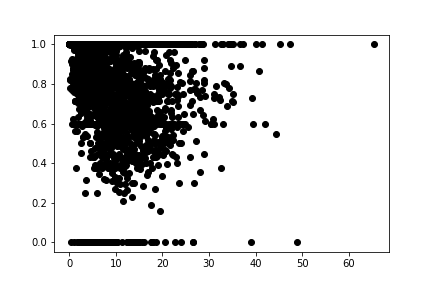
\includegraphics[width=\columnwidth]{report/img/h_clustering.png} 
  \caption{Average h-index (x axis) and global clustering coefficient (y axis)}
  \label{fig:sub-clust}
\end{subfigure}
\hfill
\begin{subfigure}{.45\columnwidth}
  \centering
  % include second image
  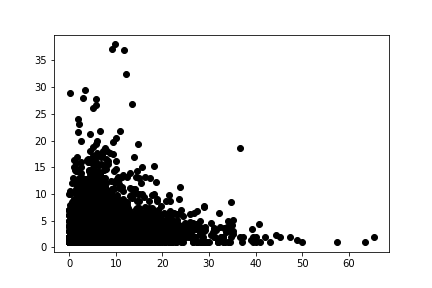
\includegraphics[width=\columnwidth]{report/img/h_deg.png}
  \caption{Average h-index (x axis) and average community degree (y axis)}
  \label{fig:sub-deg}
\end{subfigure}
\hfill
\caption{Correlation between community properties and authors' features.}\label{fig:commCorrelation}
\end{figure}

\section{Discussion}\label{sec:discussion}
% Data
Some of the collected authors' features presented a significant number of missing values, so we could not exploit all of the attributes such as research fields and list of organizations. 
% Open question
Concerning the number of citations, we had about two thirds of the total values, thus we performed a t-test for the observations in Sec \ref{sec:openQuestion}. As a future investigation, it would be interesting to enrich the analysed data to expand our knowledge about the global research community, and to group them by location, studied topics or communities. We think that a high number of intuitive and counter-intuitive correlations among them could be revealed. \\
% Link prediction
A link prediction approach in which we also consider research topics and paper titles could also be designed. For it, we would need more data. \\ 
%Future ideas
Another relevant property of networks are flows. We could exploit directness of a similar network and consider this concept in order to predict the network flows described by citations.
Concerning the achieved results, in Section \ref{sec:openQuestion} we found interesting and counter-intuitive correlations between h-index and clustering coefficient. \\
All the presented tasks highlighted the importance of computational efficiency in graph algorithms. All network analysis, link prediction and community discovery tasks have presented limits in this sense with respect to our computational resources. Indeed, the calculation of the diameter of a high-dimensional network, the task of link prediction as well as the computation of the modularity have constituted the main criticism of our work. While for the first the execution time have been considered as acceptable (see Sec. \ref{sec:networkCharacterization}), we skip the second (see Sec. \ref{sec:linkPrediction}) and we avoided the calculation of the third by means of the apposite parameters (see Sec. \ref{sec:CDweighted}).
% Community Discovery: problem of evaluation, implementation of 2nd
Concerning the adopted and implemented community discovery algorithms, our effort has been focused on the evaluation, since no ground truth was available about the network communities. Finally, more interesting results could be achieved in the opinion dynamics analysis of the network, especially by means of more executions of the Algorithmic Bias model (the most computational expensive one).

\section{Conclusions}
In our paper we collected and analysed the co-authorship network obtained by all the publications of the year 2016 available in the Microsoft Open Academic Graph.
During our work, two significant limitations raised: data quality and computational limits. Nonetheless, we analysed the network structure and we applied several state-of-the art algorithms concerning Community Discovery, Link Prediction, and Opinion Dynamics. Furthermore, we implemented an interesting (w.r.t. our network) version of CD algorithms considering both network weights and communities overlapping, but we could not exploit the proposed definition of modularity due to computational limits. Finally, some correlations have been found between network properties and authors' ones. \\
We consider that our results are useful in order to lay the groundwork for further investigations in Community Discovery and Network Diffusion applied to collaboration networks.

\bibliographystyle{ACM-Reference-Format}
\bibliography{biblio}

\end{document}